\subsection{NC efficiency estimation} \label{sec:NC_eff}
The efficiency of the NC system was decomposed into two components which one is the intrinsic efficiency and the other is the over-veto by the BVC and the CVC.
The intrinsic efficiency was measured using the $K^- p \rightarrow K0 n$ reaction with the liquid-$H_2$ target, which was the so-called MR-RUN62.
Because the over-veto by the BVC and the CVC may depend on the beam status, which was estimated using the production data. 
In this section, the intrinsic efficiency using the liquid-$H_2$ target data is explained.
The candidate of the $K^- p \rightarrow K^0 n$ reaction was searched in events detecting $\pi^+$ and $\pi^-$ by the CDS which may decay from the $K^0$.
First, $d(K^-, \pi^+ \pi^-)"n"$ events was selected as shown in Fig\ref{fig:NC_eff_Npipi_MM}.

\begin{figure}[htbp]
  \centering
  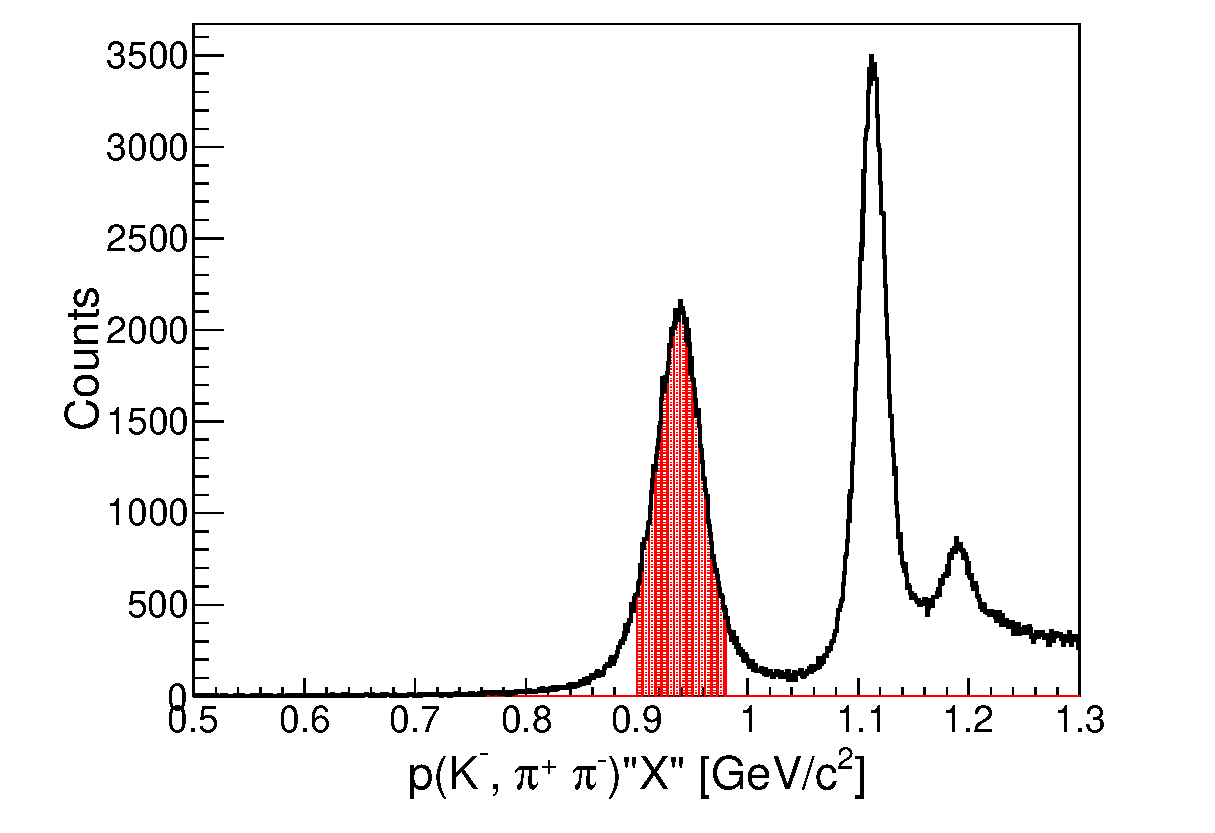
\includegraphics[width=8cm]{../pic/Run62/NC_eff/pipi_MM.eps}
  \caption{
    This figure shows $p(K^-, \pi^+ \pi^-)"X"$. $\pi^+$ and  $\pi^-$ were detected by CDS.
    A peak around 1.1GeV/c was due to $d(K^-, \pi+ \pi^-)"\Lambda"$.
    The red hatched region represents the acceptabile event as the $p(K^-, \pi^+ \pi^-)"n"$.
  }
  \label{fig:NC_eff_Npipi_MM}
\end{figure}

In this final state, the following three reactions were expected.
\begin{eqnarray}
  K^- p \rightarrow K-^0 n \label{eq:KP_K0n} \\
  K^- p \rightarrow \Sigma^+ \pi^- \label{eq:KP_pimSp} \\
  K^- p \rightarrow \Sigma^- \pi^+ \label{eq:KP_pipSm} 
\end{eqnarray}
The $\Sigma^+$ and the $\Sigma^-$ were identified from the $d(K^-, \pi^-)"X"$ and the $d(K^-, \pi^+)"X"$ as shown in the left figure of Fig \ref{fig:NC_eff_ev_id}.
For the confirmation of $K^0$ production and consistency of the momentum reconstruction, the $K^0$ reconstruction was required as shown in the right figure of Fig\ref{fig:NC_eff_ev_id}.
In the same figure, the invariant mass of $\pi^+$ $\pi^-$ was represented as a black plot.
Form that, we see $\Sigma$ rejections removed the background of the $K^0$.

\begin{figure}[htbp]
  \centering
  \begin{tabular}{cc}
    \begin{minipage}{0.65\hsize}
      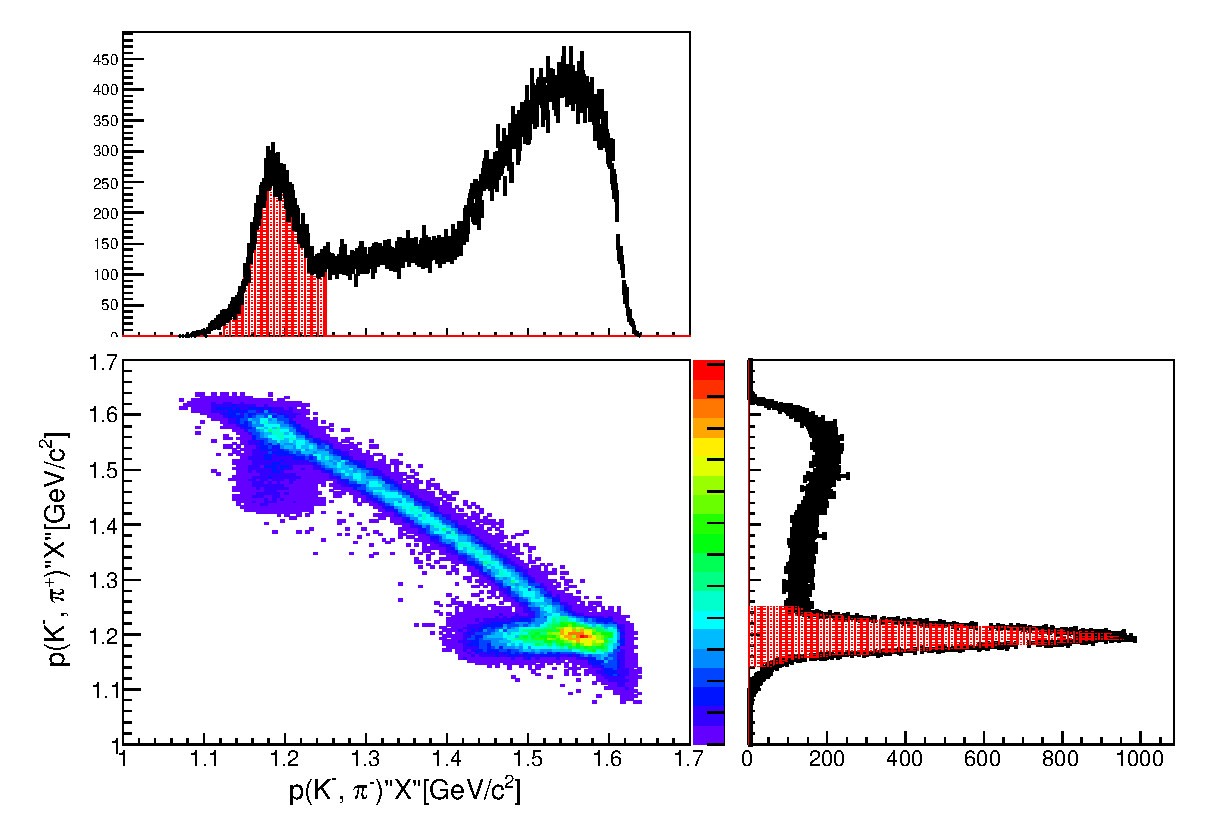
\includegraphics[width=7cm]{../pic/Run62/NC_eff/Ppim_Ppip_MM.eps}
    \end{minipage}  
    \begin{minipage}{0.45\hsize}
      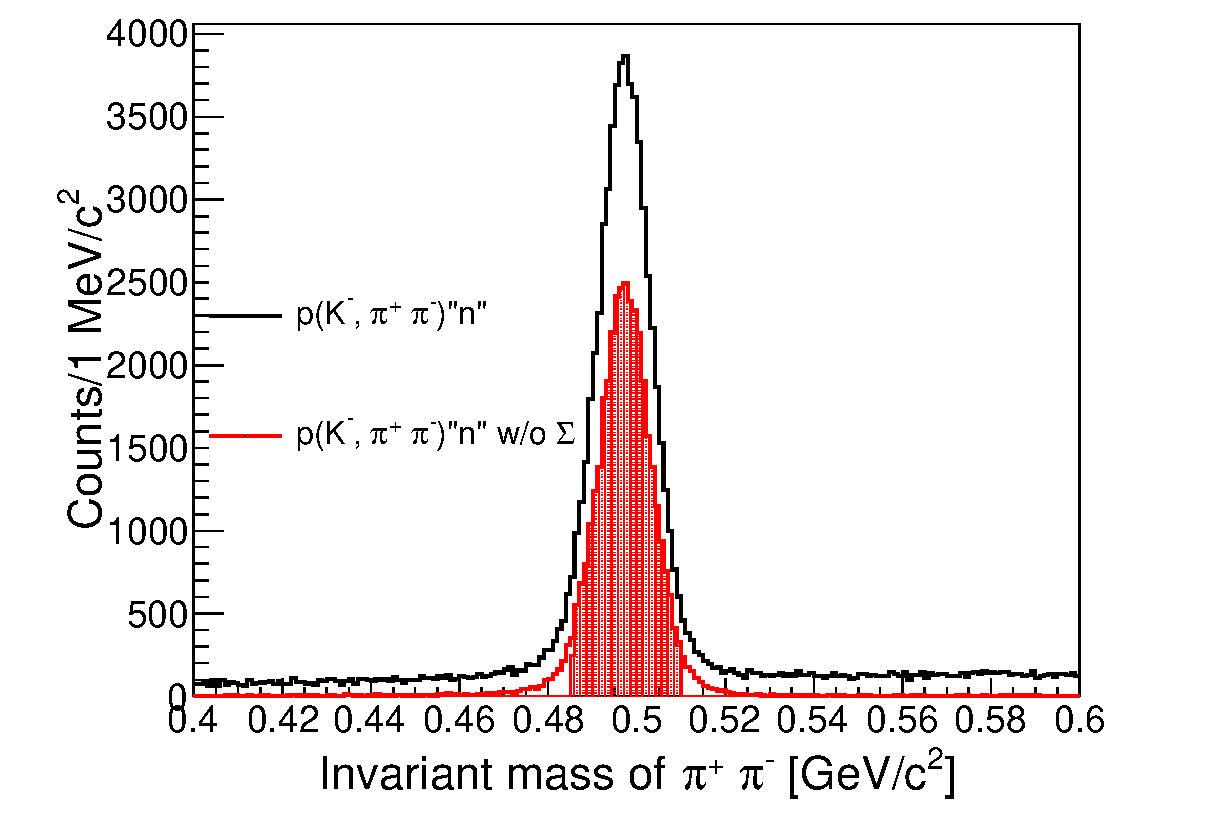
\includegraphics[width=5.5cm]{../pic/Run62/NC_eff/CDS_IM_pipi.eps}
    \end{minipage}
  \end{tabular}
  \caption{
    These figures show $K^- p \rightarrow \pi^+ \pi^- n$ event decomposition.
    The left figure shows the scatter plot of $d(K^-, \pi^+)"X"$ and $d(K^-, \pi^-)"X"$, which clearly seen $"\Sigma^-"$ and $"\Sigma^+"$, respectively.
    The red hatched region indicate these selections.
    The right figure shows the invariant mass of the $\pi^+ \pi^-$.
    The black plot indicates no selection and the red plot indicate $\Sigma$ rejected event.
    The red hatched region indicates the acceptable region as the $K^0$.
  }
  \label{fig:NC_eff_ev_id}
\end{figure}

The hit position at the NC of the missing neutron comes from the reaction that was reconstructed from the momenta of beam, $\pi-+$, and $\pi^-$.
That was drawn in the Fig\ref{fig:NC_hitpos}, in which the left figure shows as all events and the right figure shows events that have the NC signal.
In the fight figure, the NC profile is clearly seen.

Because this estimation is the measurement of the intrinsic NC efficiency, the trigger event was used the events had no signal in the CVC and the PC.
The NC efficiencies were evaluated in several regions at the NC, which was shown in Fig\ref{fig:NC_eff}.
The NC efficiencies were saturated at the NC size$=-20cm$, so the NC efficiency was estimated at $0.317 \pm 0.016$ at this condition.

\begin{figure}[htbp]
  \centering
  \begin{tabular}{cc}
    \begin{minipage}{0.5\hsize}
      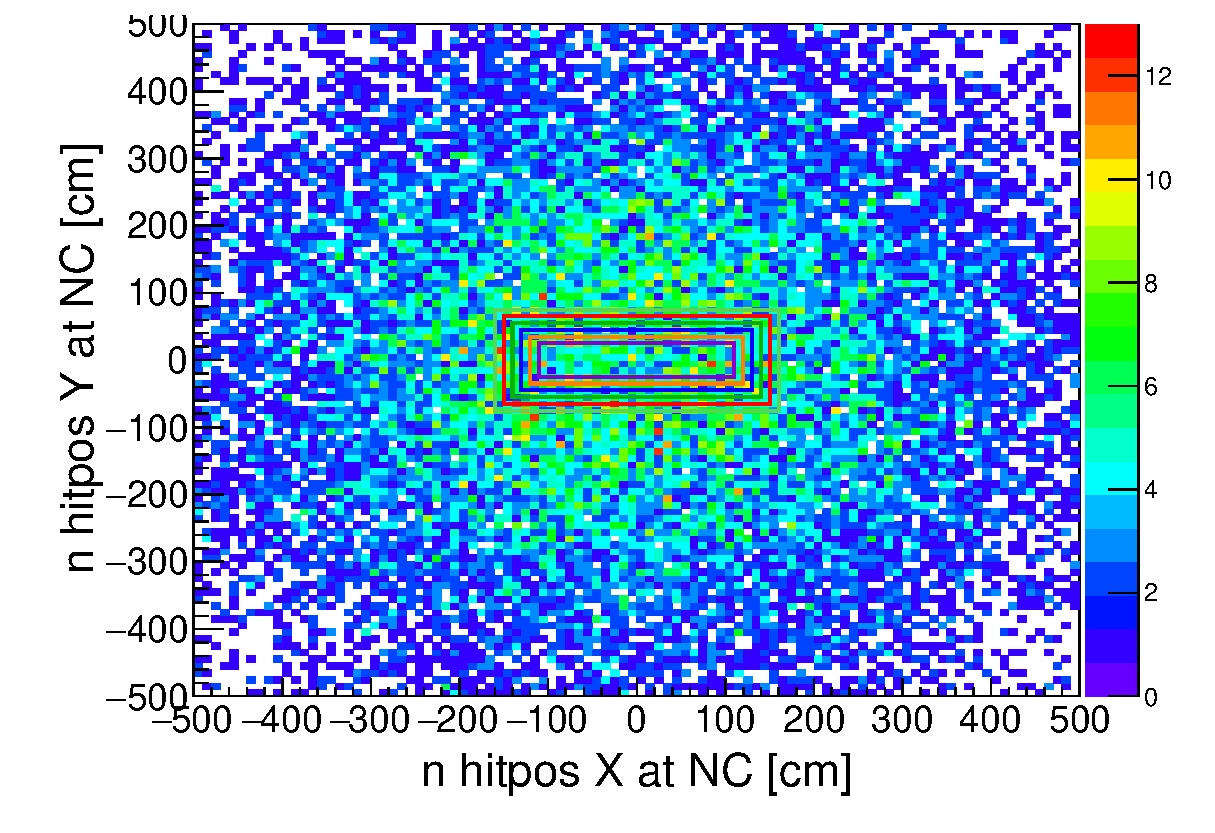
\includegraphics[width=6cm]{../pic/Run62/NC_eff/hitpos.eps}
    \end{minipage}
    \begin{minipage}{0.5\hsize}
      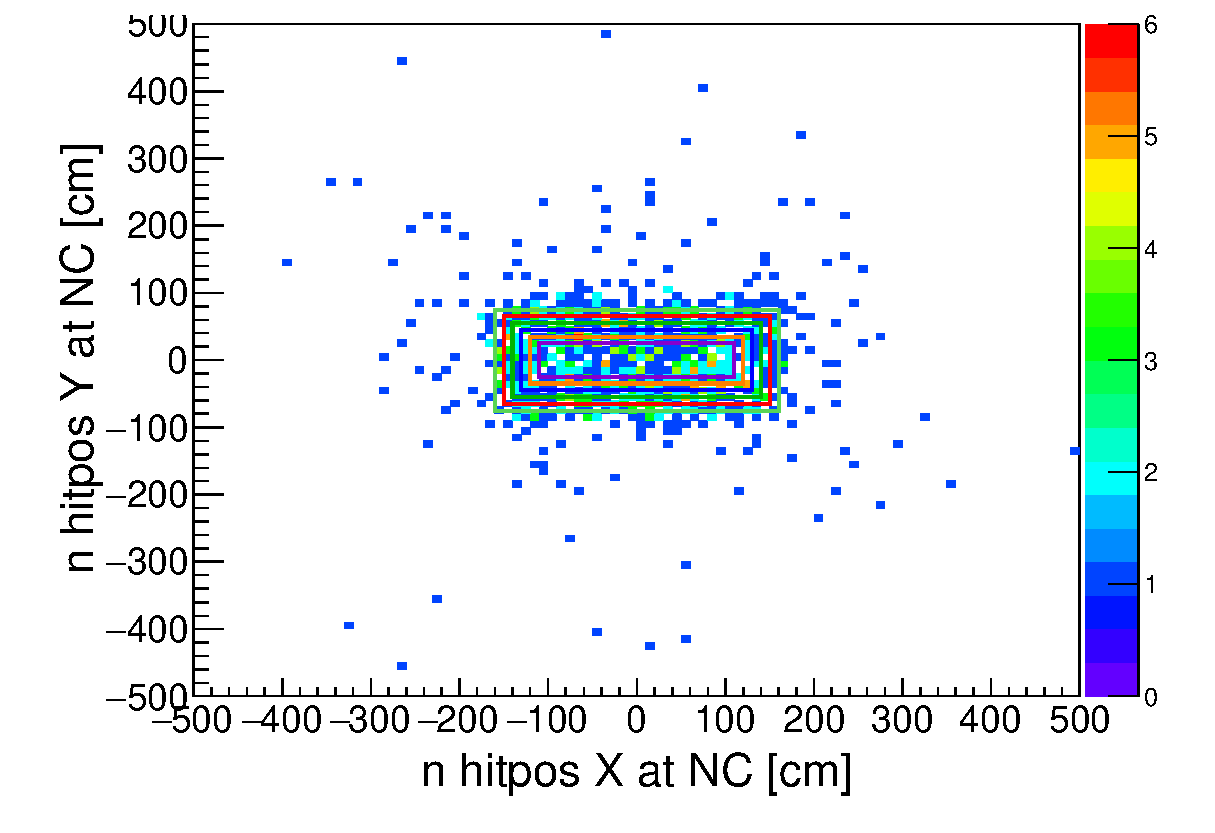
\includegraphics[width=6cm]{../pic/Run62/NC_eff/hitpos_whit.eps}
    \end{minipage}
  \end{tabular}
  \caption{
    These figures show the calculated hit position at the NC from the reconstructed momentum of the $p(K^-, \pi^+ \pi^-)"n"$.
    The left figure indicates all events and the right figure indicates with the NC signal.
    The box indicates the NC size. % To do 枠線を取り除く
  }
  \label{fig:NC_hitpos}
\end{figure}
\begin{figure}[htbp]
  \centering
  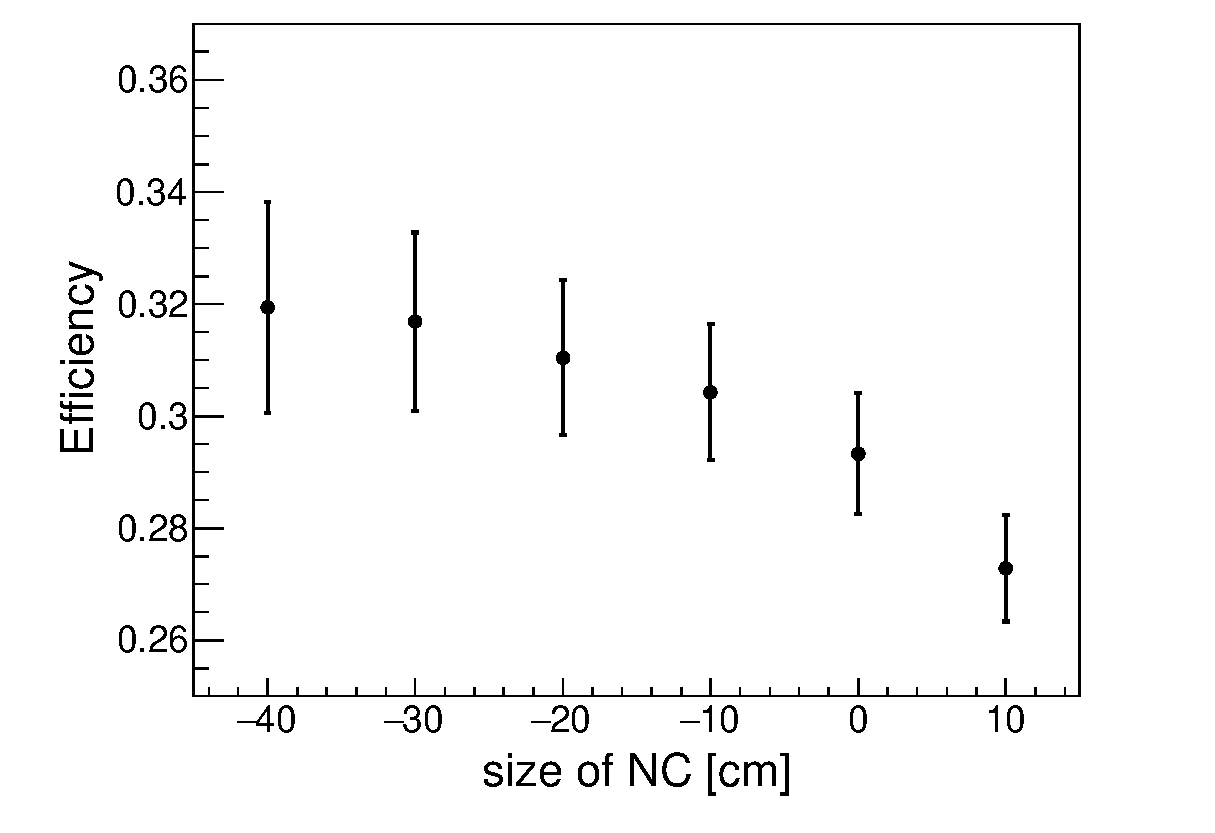
\includegraphics[width=8cm]{../pic/Run62/NC_eff/NC_eff.eps}
  \caption{
    This figure indicates the relation of NC efficiencies and selected regions.
    Error bars represents statistic errors.
  }
  \label{fig:NC_eff}
\end{figure}
